\documentclass{article}

\usepackage{graphicx}
\usepackage{amsmath, amsfonts, amsthm, amssymb}
\usepackage{xspace}
\usepackage{tikz}
\usepackage{pgf,tikz}
\usepackage{mathrsfs}
\usepackage{caption}
\usetikzlibrary{arrows}
\usetikzlibrary{intersections}
\usetikzlibrary{patterns, snakes}
\usepackage{float}
\usepackage{multicol}
\usepackage{hyperref}

\usepackage[backend=bibtex,style=verbose-trad1, citestyle=numeric]{biblatex}


\newcommand\dd{{2-Dimensional}\xspace}
\newcommand\ddd{{3-Dimensional}\xspace}
\newcommand\ru{\hat{\mathbf{r}}\xspace}
%\newcommand\rv{\hat{\mathbf{r}}\xspace}
\newcommand\cpv{\overrightarrow{CP}\xspace}

\newcommand\sina{2 r_p\frac{\sqrt{\left|\cpv\right|^2 - r_p^2}}{\left|\cpv\right|^2}}
\newcommand\cosa{ \frac{\left|\cpv\right|^2 - 2 r_p^2}{\left|\cpv\right|^2}}
\newcommand\sinah{\frac{r_p}{\left|\cpv\right|}}
\newcommand\cosah{\frac{\sqrt{\left|\cpv\right|^2 - r_p^2}}{\left|\cpv\right|}}

\newcommand\proj[2]{\frac{#1 \cdot #2}{\left|#2\right|^2} #2}

\newcommand\xp{x\prime\xspace}
\newcommand\yp{y\prime\xspace}
\newcommand\vp{v\prime\xspace}

\newcommand{\bb}[1]{\mathbf{#1}}

\title{Projecting Spherical Objects onto a 2-Dimensional plane within 3-Dimensional Space}


\date{}
\begin{document}
\maketitle
\tableofcontents
\section{Scenario}

	\subsection{Introduction}
		Consider \ddd space containing objects we will define as spheres of any size. Within this space, we will have a point of
		observation, called the camera. The camera itself is a singular point, however at a fixed distance from the camera, in a direction given by a
		unit vector $\ru$ , is a \dd plane
		representing the screen of the computer running the simulation. The location of the camera and each object will be given as a vector:
		$$P = \begin{pmatrix}x_P\\y_P\\z_P\end{pmatrix}, C = \begin{pmatrix}x_C\\y_C\\z_C\end{pmatrix}, \hat{\mathbf{r}} = \begin{pmatrix}x_r\\y_r\\z_r\end{pmatrix}:|\ru|=1$$
	%	Likewise, the position of an object in space will be given as:


		In Figure \ref{fig:proj3d}, the line perpendicular to the plane through C is parallel to $\ru$, and the distance from the camera to the screen will be
		defined as $S_d$.
	\subsection{Projecting spheres onto a plane}
		Projecting a spherical object onto a \dd plane, if the plane is not perpendicular to the vector between the camera and the object, will produce a conic section, ie, an ellipse. This is essentially the definition of a conic section, the intersection of a \dd plane and a cone extending from the camera at $C$ to the object at $P$, made up of the tangents that join them.
		See figure \ref{fig:proj3d} for a visualisation.
		Such an ellipse will have certain properties, such always being aligned so that the line through the major axis passes through the centre of the screen, meaning there are three unknowns:
	\begin{itemize}
		\item The length of the minor axis
		\item The length of the major axis
		\item The $x$ and $y$ position of the object \textit{on the screen}
	\end{itemize}

	\begin{figure}
		\includegraphics[width = 12cm]{Fig1.PNG}
		\caption{Projection of a sphere onto a \dd plane.}
		\label{fig:proj3d}
		\includegraphics[width = 12cm]{Fig2.PNG}
		\caption{View of the ellipse looking onto the plane (from underneath)}
		\label{fig:proj2d}
	\end{figure}

	\paragraph{}
	In Figure \ref{fig:proj3d}, the plane shown by the grid represents the screen, the red sphere and the blue dot at $C$ correspond to the object in space and
	the camera, also in space, respectively. It is clear how the projection of the sphere onto the plane would produce a conic section, and it is
	worth noting that if an observer were to observe this ellipse fom $C$, the ellipse would appear to be a circle. In the example shown in the
	figure, the object is so far from the centre of the screen (marked by $S_C$) relative to the distance of the camera from the screen that the
	projection would place the ellipse well outside the physical bounds of the screen, and in reality the eccentricity of the projections would be very low.
	\paragraph{}
	Figure \ref{fig:proj2d} shows what the projection would look like on the screen, as it would appear looking perpendicular towards the plane from
	underneath it. The perpendicular lines are shown for reference.


\section{Finding the Shape of the Ellipse Using Geometry}
	Calculating the lengths of the major and minor axis of the projection is fairly simple, and involves a bit of trigonometry.
	\subsection{Finding the Length of the Major Axis}
	As the major axis is aligned with the origin - the centre of the screen - there is no use in breaking the problem into $x$ and $y$
	components, it is better to look at a cross sectional diagram parrallel with the major axis, as shown in Figure \ref{fig:majorAxis}.
	In the diagram, the displacement vector $\overrightarrow{CP}$, the vector $\hat{\mathbf{r}}$, the length of $CS_C$ and the radius of the
	particle $r_p$ are the only known variables. The angle $\theta$ is going to be the angle between $\ru$ and $\cpv$.
	\begin{figure}
		\includegraphics[width = 12cm]{Fig3.pdf}
		\caption{Diagram of the projection of a circle onto a line, in this case, the red line $a$ is equivalent to the major axis in the \ddd case.}
		\label{fig:majorAxis}
	\end{figure}
%	\paragraph{}
	Thus, to find theta, we use the dot product of the two vectors:
	$$
	\ru \cdot \cpv = |\ru| |\cpv| \cos{\theta} $$ $$
	\cos{\theta} = \frac{\ru \cdot \cpv}{|\ru||\cpv|}
	$$
	\begin{equation}
		\cos{\theta} = \frac{\ru \cdot \cpv}{|\cpv|}
	\end{equation}
%	\paragraph{}
	Since $\ru$ is defined to have a length of 1. Then,
	$$\cos{\theta} = \frac{S_D}{|CS_P|} $$
	\begin{equation}
		\left|C S_P\right| = \frac{S_D}{\cos{\theta}}
	\end{equation}
	\paragraph{}
	Thus we now know both the angle of the particle from the centre of the screen and the distance from the origin of the camera to the
	projection. This will allow us to also calculate $|S_C S_P|$, the distance from the centre of screen to the centre
	of the projection, although isn't needed for this part of the problem, but will be used later on.

	$$\left| \overrightarrow{S_C S_P} \right| =\sqrt{ \left|C S_P\right|^2 - S_D ^2}$$

	\paragraph{}
	Now, to find the length of $a$, we will also need the angle $\alpha$, which is the angle between the two tangents joining the circle at $P$
	to the camera at $C$. This is found using the right angled triangles on either side of $\cpv$.
	$$\sin\left(\frac{\alpha}{2}\right)  = \frac{r_p}{\left|\cpv\right|},\text{   } \cos{\left(\frac{\alpha}{2}\right)} = \frac{\sqrt{\left|\cpv\right|^2 - r_p^2}}{\left|\cpv\right|} $$
	\pagebreak
	\begin{multicols}{2}
	\begin{align*}
		\cos{\alpha} & = \cos^2{\frac{\alpha}{2}} -  \sin^2{\frac{\alpha}{2}}\\
					& = \frac{\left|\cpv\right|^2 - r_p^2}{\left|\cpv\right|^2} - \frac{r_p^2}{\left|\cpv\right|^2}\\
					& = \frac{\left|\cpv\right|^2 - 2 r_p^2}{\left|\cpv\right|^2}
	\end{align*}
	\columnbreak
	\begin{align*}
		\sin{\alpha} & = 2 \sin{\frac{\alpha}{2}} \cos{\frac{\alpha}{2}}\\
					& = 2 r_p \frac{\sqrt{\left|\cpv\right|^2 - r_p^2}}{\left|\cpv\right|^2}
	\end{align*}
	\end{multicols}
	\begin{multicols}{2}
	\begin{equation}
		\therefore \cos{\alpha} = \frac{\left|\cpv\right|^2 - 2 r_p^2}{\left|\cpv\right|^2}
	\end{equation}
	\columnbreak
	\begin{equation}
		\therefore \sin{\alpha} = 2 r_p\frac{\sqrt{\left|\cpv\right|^2 - r_p^2}}{\left|\cpv\right|^2}
	\end{equation}
	\end{multicols}
	\paragraph{}
	Now the length of $a$ can be calculated from the difference in the distance from $S_C$ to the closest tangent line and the furthest tangent 	line. In the following working, we will call those distances $d_1$ and $d_2$ for the shortest distance and longest distance respectively,
	such that $d_2 - d_1 = a$.
	$$  d_2 =  \tan{\left(\theta + \frac{\alpha}{2}\right)} S_D $$
	$$  d_1 =  \tan{\left(\theta - \frac{\alpha}{2}\right)} S_D $$
	\begin{align*}
		a = d_2 - d_1 & = S_D \left(\tan{\left(\theta + \frac{\alpha}{2}\right)} - \tan{\left(\theta - \frac{\alpha}{2}\right)} \right) \\
		& = S_D\left(\frac{\sin{\left(\theta + \frac{\alpha}{2}\right)}}{\cos{\left(\theta + \frac{\alpha}{2}\right)}}
				    - \frac{\sin{\left(\theta - \frac{\alpha}{2}\right)}}{\cos{\left(\theta - \frac{\alpha}{2}\right)}}\right)    \\
		& = S_D \frac{\sin{\alpha}}{\cos{\left(\theta + \frac{\alpha}{2}\right)} \cos{\left(\theta - \frac{\alpha}{2}\right)}} \\
		& = S_D \frac{\sin{\alpha}}{\cos^2{\theta} \cos^2{\frac{\alpha}{2}} - \sin^2{\theta} \sin^2{\frac{\alpha}{2}}} \\
	\end{align*}
	All terms of which are known. And so we have,
	\begin{equation}
		a =  S_D \frac{\sin{\alpha}}{\cos^2{\theta} \cos^2{\frac{\alpha}{2}} - \sin^2{\theta} \sin^2{\frac{\alpha}{2}}}
	\end{equation}
	There are other ways to find this length, some of them are probably easier. Expanding this to be in terms of the known variables gives:
	\begin{equation*}
		a = S_D  \left(\frac{2 r_p \left(\left|\cpv\right|^2-r_p^2\right)^{(3/2)}}{\left|\cpv\right|^4  \cos^2{\theta}}-
		\frac{r^2 \sin^2{\theta}}{\left|\cpv\right|^2}\right)
	\end{equation*}
	Or as code:
	\begin{verbatim}
		a = SD * (2 * rp * (CP**2 - rp**2)**(3/2) /
		    (CP**4 * cos(theta)**2) - sin(theta)**2 * rp**2 / CP**2)
	\end{verbatim}

	\subsection{Finding the Length of the Minor Axis}
	\paragraph{}
	Finding the length of the minor axis, $b$, is much simple than the major axis. The minor axis is orthogonal to the line joining the camera
	and the object, so methods like the ones used in the previous section won't be necessary.
	\begin{figure}[H]
		\includegraphics[width = 14cm]{Fig4.pdf}
		\caption{Diagram of the projection of a circle onto a plane where the red line represents the minor axis of the ellipse.}
		\label{fig:minorAxis}
	\end{figure}
	\paragraph{}
	From Figure \ref{fig:minorAxis}:
	\begin{align*}
		\tan{\frac{\alpha}{2}} & = \frac{r_p}{\sqrt{\left|\cpv\right|^2 - r_p^2}} \\
		b & = 2 S_D \tan{\frac{\alpha}{2}}
	\end{align*}
	\paragraph{}
	And so we have:
	\begin{equation}
		b = S_D \frac{2 r_p}{\sqrt{\left|\cpv\right|^2 - r_p^2}}
	\end{equation}
	As code:
	\begin{verbatim}
		b = SD * 2 * rp / (CP**2 - rp**2)**(1/2)
	\end{verbatim}
	Thus we have the major and minor axis of the ellipse. Now two of the three unknowns have been calculated, all that remains is to find the position of the ellipse on the screen.

\section{Finding the Position of the Ellipse on the Screen}
	\subsection{Vector Geometry}
	To find the x and y component of the position on the screen, vector geometry is needed. The most important function we will use is the
	projection of one vector onto another. Defined as:
	$$ \text{Proj}_{\mathbf{b}}\mathbf{a} = \frac{\mathbf{a} \cdot \mathbf{b}}{|\mathbf{b}|^2} \mathbf{b} $$
	The result gives you the projection of $\mathbf{a}$ onto $\mathbf{b}$. When just distances are needed, we divide
	by the unit vector of $\mathbf{b}$, ie $\frac{\mathbf{b}}{|\mathbf{b}|}$ to get
	$$ \left|\text{Proj}_\mathbf{b} \mathbf{a}\right| = \frac{\mathbf{a} \cdot \mathbf{b}}{|\mathbf{b}|} $$

	Vector projection can infact be thought of to be defined as multiplying the above scalar value by the unit vector of the vector being projected onto.
	\paragraph{}
	To get the $x$ and $y$ components, consider two vectors $\yp$ and $\xp$, both parallel to the plane of the screen but:
	\begin{itemize}
		\item $\xp$ is parallel to the $x$-axis of the screen, meaning it is orthogonal to both the vector $\overrightarrow{C S_C}$ and the global $y$-axis.
		\item $\yp$ is parallel to the $y$-axis of the screen, meaning it is orthogonal to both the vector $\overrightarrow{C S_C}$ and $\xp$.

	\end{itemize}
	The lengths of $\xp$ and $\yp$ are irrelevant, only their directions are important. Thus, from their definitions,
	\begin{align*}
			\xp & = \overrightarrow{C S_C} \times \begin{pmatrix} 0\\1\\0 \end{pmatrix}\\
			     & = S_D \begin{pmatrix}x_r\\y_r\\z_r\end{pmatrix} \times \begin{pmatrix} 0\\1\\0 \end{pmatrix}\\
			    & = \begin{pmatrix} -S_D z_r\\ 0\\ S_D x_r \end{pmatrix}
	\end{align*}
	\begin{equation}
		\therefore \xp = \begin{pmatrix} -z_r \\0 \\x_r\end{pmatrix}
	\end{equation}
	And,
	\begin{align*}
		\yp & = \overrightarrow{C S_C} \times \xp \\
		     & = S_D  \begin{pmatrix}x_r\\y_r\\z_r\end{pmatrix} \times \begin{pmatrix} -z_r\\ 0\\ x_r \end{pmatrix} \\
		     & = S_D \begin{pmatrix} x_r y_r \\ -\left({x_r}^2 + {z_r}^2\right) \\ z_r y_r \end{pmatrix}
	\end{align*}
	\begin{equation}
		\therefore \yp = \begin{pmatrix} x_r y_r \\ -\left({x_r}^2 + {z_r}^2\right) \\ z_r y_r \end{pmatrix}
	\end{equation}
	\paragraph{}

	\begin{figure}
		\centering
		\includegraphics[width = 12cm]{Fig5.pdf}
		\caption{The triangle $Z S_C S_P$ lies on the plane of the screen, perpendicular to $\hat{\mathbf{r}}$. The point P will lie on any point on the ray through $\protect\overrightarrow{C S_P}$ represented by the dotted line.}
		\label{fig:screen}
	\end{figure}

	\paragraph{}
	Now that we have the $x$ and $y$ axes of the screen, the $x$ and $y$ components of the position of particle are the respective lengths of the projection of $\overrightarrow{S_C S_P}$ onto $\xp$ and $\yp$.
	We recall $\overrightarrow{S_C S_P}$ to be:
	\begin{align*}
		\overrightarrow{S_C S_P} & = S_P - S_C \\
		& = C S_P - C S_C \\
		& = \frac{\left|\overrightarrow{CP}\right|}{\left|\overrightarrow{C S_P}\right|} \overrightarrow{CP} - S_D \hat{\mathbf{r}}
			& \left|\overrightarrow{C S_P}\right| \text{is defined in equation (2).} \\
	\end{align*}
	Therefore,
	$$x = \frac{\overrightarrow{S_C S_P} \cdot \xp}{\left|\xp\right|} $$
	$$y = \frac{\overrightarrow{S_C S_P} \cdot \yp}{\left|\yp\right|} $$

\section{Rotation of the $x$ and $y$ axes about each other}
	\paragraph{}
	In order to rotate the screen, two methods can be used. Either the vector $\ru$ be rotated and the $x, y$ axes $\xp, \yp$ be recalculated for each draw,
	or the $x$ and $y$ axes be rotated and $\ru$ be recalculated. The latter is preferable as the first method restricts the orientation of the screen such that $\yp$ always passes through the $y$-axis.
	If the axes can be rotated independently of each other then the user is able to orientate the screen in any direction,
	and rotation of the screen about it's $z$-axis becomes possible and feasible. However, to rotate a vector about another vector is no trivial task.
	\subsection{Rotation of a vector about another vector}
	\paragraph{}
	Consider the vectors;
	\begin{itemize}
	\item $a$: The axis of rotation
	\item $v$: The initial vector to be rotated
	\item $\vp$: The rotation of $v$ about $a$
	\end{itemize}
	\paragraph{}
	For our situation, $a$ and $v$ would be perpendicular, making the problem slightly easier. Although, it is useful to see the general solution.
	\paragraph{}
	The vector $v$ can be broken down into $v_{\parallel a} + v_{\perp a}$, the component along $a$ and the component orthogonal to $a$.
	$v_{\parallel a}$ is simply the projection of $v$ onto $a$,
	$$v_{\parallel a} = \proj{a}{v}$$
	And the orthogonal part is then just $v - v_{\parallel a}$
	$$v_{\perp a} = v - \proj{a}{v}$$

	\paragraph{}
	Now, consider the plane orthogonal to $a$, a vector on this plane can hence be made by the linear combination of
	$x_1 v_{\perp a} + x_2 a \times v$, both vector components of which are orthogonal to $a$.
	Thus, to get a rotation by a specific angle $\theta$, let,
	$$x_1 = \frac{\cos{\theta}}{\left| v_{\perp a} \right|} \text{   and   } x_2 = \frac{\sin{\theta}}{\left| a \times v \right|}$$
	Such that the component of the resulting vector on this plane is
	$$\vp_{\perp a} = \left|v_{\perp a} \right| \left( \frac{\cos{\theta} v_{\perp a}}{\left| v_{\perp a} \right|}
					+ \frac{\sin{\theta} (a \times v)}{\left|a \times v\right|}\right) $$
	The final result can be given by $\vp = \vp_{\perp a} + v_{\parallel a}$, therefore;
	\begin{equation}
	\vp =  \left|v_{\perp a} \right| \left( \frac{\cos{\theta} v_{\perp a}}{\left| v_{\perp a} \right|}
					+ \frac{\sin{\theta} (a \times v)}{\left|a \times v\right|}\right) + \proj{a}{v}
	\end{equation}
	\paragraph{}
	As stated, in our case $v_{\parallel a} = 0$, and so the last term in the equation drops out.
	Thus to rotate $\xp$ about $\yp$ we substitute $a = \yp$ and $v = \xp$, and vice versa.

\subsection{Re-orientating $\ru$ to the new screen}

Now, we are able to rotate the vectors about each other, although we haven't changed $\ru$ yet. By definition, $|\ru| = 1$, but is parallel to the normal through $\xp$ and $\yp$ (although in the code the length isn't always assumed to be 1 as a safety net).
	Additionally, $S_D$ is fixed and does not change, so we are easily able to find the new direction of $\ru$ and thus the new position of the screen.
	\paragraph{}
	Expanding on their definitions,
	$$\ru \parallel \xp \times \yp$$
	$$\ru = \frac{\xp \times \yp}{\left|\xp \times \yp\right|}$$
	Note that this requires $\xp$ and $\yp$ to be in the direction of the right and the top of the screen respectively.

\section{Simulation Using the Leapfrog Method}
The most obvious way to simulate an n-body universe is to calculate the acceleration of each particle at a certain time, apply that to the velocity of the particle using a specified time step, then apply the new velocity to the position of the particle.
\begin{align*}
	\mathbf{a}_i &= \mathbf{F}_i/m\\
	\mathbf{v}_{i+1} &= \mathbf{a}_i \Delta t\\
	\mathbf{p}_{i+1} &= \mathbf{v}_{i+1} \Delta t\\ \text{or  }
	\mathbf{p}_{i+1} &= \mathbf{v}_i \Delta t
\end{align*}
\paragraph{}
However this method has a significant error, which gets much larger as the time step increases.
The leapfrog approach is a more accurate method, and differs from the previous method in that it uses the velocity at one half step ahead of the current time.
\begin{align*}
	\mathbf{v}_{i+1/2} &= \mathbf{v}_{i-1/2} + \mathbf{a}_i \Delta t  \\
	\mathbf{p}_{i+1}    &= \mathbf{p}_i + \mathbf{v}_{i + 1/2} \Delta t
\end{align*}
In a parabolic position time scenario, the approximation provides an exact result, with 100\% accuracy.
In an n-body simulation this is essentially never the case but it is still a good approximation, as shown in the figure.\\
\begin{center}
\begin{tikzpicture}
	\draw[<->] (0, 5) -- (0, 0) -- (5, 0);
	\draw [name path = curve] (0,1) to [out = 10, in = 250] (4.5, 5);
	\path [name path = x0] (1,0) -- (1,5);
	\path [name path = x1] (4,0) -- (4,5);
	\path [name path = xh] (2.5, 0) -- (2.5, 5);
	\node [label = -90:$x_0$] at (1, 0) {};
	\node [label = -90:$x_1$] at (4, 0) {};
	\path [name intersections={of = curve and x0, by=y0}];
	\path [name intersections={of = curve and x1, by=y1}];
	\draw [line width=0.1] (1,0)--(y0);
	\draw [line width=0.1] (4,0)--(y1);
	\draw [<->] (1,-0.7) -- (4, -0.7) node [pos=0.5, anchor=north] {h};
%	\draw [decoration={brace, mirror, raise = 0.5}, decorate] (1, -1) -- (4, -1) node [pos=0.5, anchor=north, yshift=-0.5] {h} ;

\end{tikzpicture}
\end{center}
\subsection{Starting the simulation}
	\paragraph{}
	The main difficulty with this method is starting the process, where normally the position and velocities are given at a single instant, not a half step difference.
	To start the simulation, we must offset the velocity using the normal methods shown at the start of the section.
	ie, if $v_0$ and $x_0$ are given, then;
	$$v_{1/2} = v_0 + a_0 \frac{\Delta t}{2}$$
	This makes it difficult to change the time step in the simulation, as the offset at the start is based on the initial time step.
	To do so, we have to first remove the offset between the position and velocity, one way to do this is to first subtract $a_i \frac{\Delta t_0}{2}$ from, then adding $a_i \frac{\Delta t_1}{2}$ to the current $v$, where $\Delta t_0$ and $\Delta t_1$ are the previous and new time steps respectively.

\subsection{Using matrix mathematics to perform faster calculations}
	Generally using a static n-dimensional array as a matrix will be
	faster than using a dynamic n-dimensional list. This is especially
	the case with Numpy's arrays compared to the native python lists.

	To make calculations we require the following arrays to be known at all times:
	\begin{itemize}
		\item $\bb P_N \in \mathbb{R}^{N \times 3} \to$ Array of position vectors.

		\item $\bb R \in \mathbb{R^N} \to $ Array of radii of particles.

		\item $\bb M \in \mathbb{R^N} \to $ Array of masses of particles.
	\end{itemize}
	Where $N$ is the number of particles. For a calculation such as standard
	gravitational attraction, we would perform the following particle for each particle.
	Here the individual particle we are simulating for is as position $\bb P$,
	with mass $M$ and radius $R$.
	\begin{align*}
		\intertext{Find the distance to each other particle:}
		\bb D_N &= \bb P_N - \{\bb P \} \\
		\intertext{(The braces indicate the subtraction is for each element in the matrix $\bb P_N$)}
		\intertext{The absolute distances are given by:}
		\bb D &= |\bb D_N| = \{|\bb x| \forall \bb x \in \bb D_N \}
		\intertext{For the force:}
		\bb F_N &=  G M \odot \bb M \odot (\bb D_N) \oslash (|\bb D|^3) \\
		\intertext{Where $\odot, \oslash$ are element wise multiply and divide respectively.
							Also note that cubic power at the right is element wise aswell.}
		\intertext{Now we sum the forces to get the net force:}
		\bb F &= \sum_{n = 0}^{N} \bb F_{N_n} \\
		\intertext{The acceleration is simply derived from $\bb F = m \bb a$, however it
							would be fine to simply remove the mass of the particle at the start
							in this case to directly calculate acceleration instead of force.}
		\intertext{We also want to check for collisions. Lets consider a vector $\bb A$
							containing the `altitude' of each particle, ie the surface-surface distance.}
		\bb A &= \bb D - \bb R - \{R\} \\
		\bb B_\mathrm{collision} &= \{\bb A < 0\}
		\intertext{Where $\bb B$ is a boolean vector where a value of True indicates that
								our current particle is colliding with the particle at that index.}
	\end{align*}


\section{Drawing Crescents on Bodies}
	\paragraph{}To draw a crescent on a body, we first imagine drawing a disc that represents the boundary between the surface of the body illuminated and the surface of the body in darkness.
	The radius of this disk is given by:

	$$r = R_2\sqrt{2\left(1 - \cos{2\theta}\right)}$$
	where $\theta$ is given by;
	$$\cos{\theta} = \frac{R_1 - R_2}{d}$$
	where $R_1$ and $R_2$ are the radii of the parent body (eg. the sun) and the child body (eg. the earth) respectively. $d$ is the distance between the centre of each body, as shown in Figure \ref{fig:crescentRadius}.
\begin{figure}
	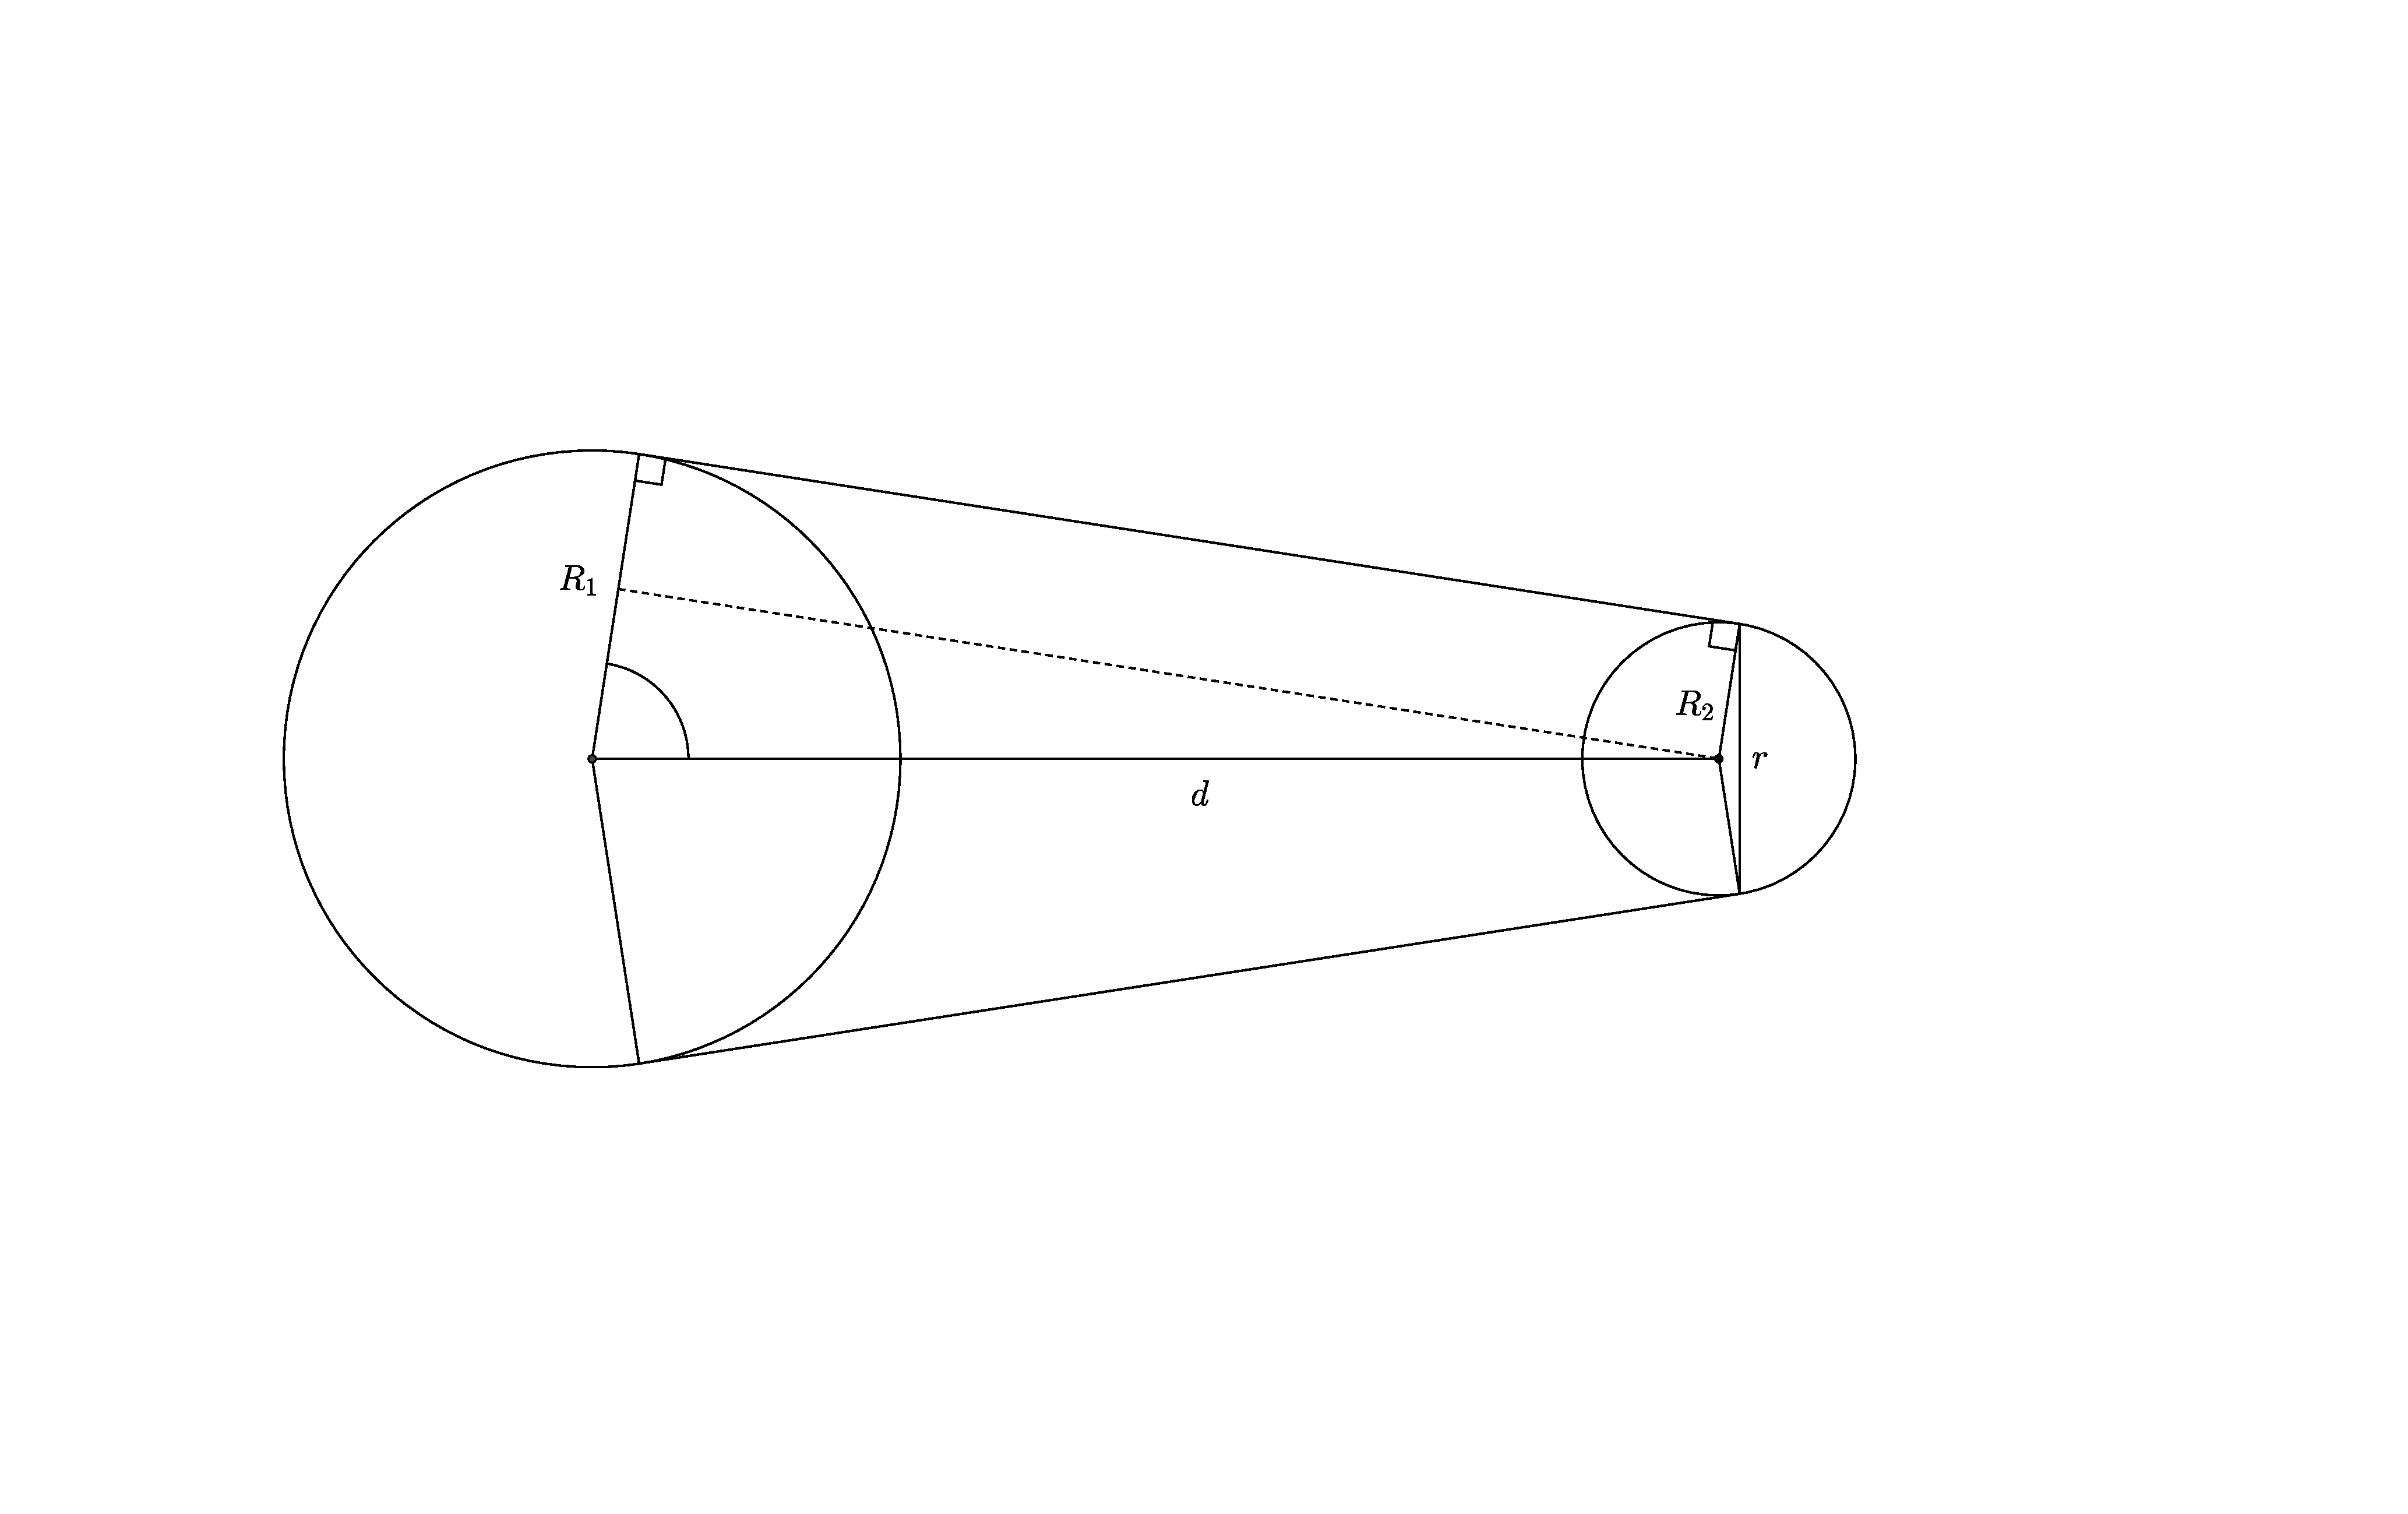
\includegraphics[width = 14cm]{CrescentRadius.pdf}
	\caption{A cross section representing the radius of the boundary disc between illuminated and non illuminated surface, the disc is the line of length $2r$, such that r is the radius of that disc.}
	\label{fig:crescentRadius}
\end{figure}




\end{document}
